\documentclass[conference]{IEEEtran}

\usepackage{cite}
\usepackage{amsmath}
\usepackage{graphicx}
\usepackage{booktabs}
\usepackage{url}
\usepackage{tikz}
\usetikzlibrary{arrows.meta,positioning,calc}
\usepackage{listings}

% generated by make_paper_assets.py - do not edit
\newcommand{\res}[1]{\csname res@#1\endcsname}
\expandafter\def\csname res@loc_lexer\endcsname{369}
\expandafter\def\csname res@loc_parser\endcsname{982}
\expandafter\def\csname res@loc_semantic\endcsname{657}
\expandafter\def\csname res@loc_bytecode\endcsname{851}
\expandafter\def\csname res@loc_vm\endcsname{563}
\expandafter\def\csname res@loc_common\endcsname{49}
\expandafter\def\csname res@loc_main\endcsname{167}
\expandafter\def\csname res@loc_total\endcsname{3{,}638}
\expandafter\def\csname res@loc_opcodes\endcsname{34}
\expandafter\def\csname res@tests_total\endcsname{62}
\expandafter\def\csname res@tests_failed\endcsname{0}
\expandafter\def\csname res@tests_run\endcsname{17}
\expandafter\def\csname res@tests_bytecode\endcsname{17}
\expandafter\def\csname res@tests_reject\endcsname{28}
\expandafter\def\csname res@tests_examples\endcsname{17}
\expandafter\def\csname res@tests_rejected_programs\endcsname{28}
\expandafter\def\csname res@linux_total\endcsname{62}
\expandafter\def\csname res@linux_gpp\endcsname{15.2.0}
\expandafter\def\csname res@audit_total\endcsname{20}
\expandafter\def\csname res@audit_critical\endcsname{4}
\expandafter\def\csname res@audit_high\endcsname{8}
\expandafter\def\csname res@audit_medium\endcsname{8}
\expandafter\def\csname res@show_source_lines\endcsname{161}
\expandafter\def\csname res@show_functions\endcsname{11}
\expandafter\def\csname res@show_tokens\endcsname{979}
\expandafter\def\csname res@show_ast_nodes\endcsname{704}
\expandafter\def\csname res@show_instructions\endcsname{732}
\expandafter\def\csname res@show_executed\endcsname{230{,}016}
\expandafter\def\csname res@show_check_null\endcsname{14}
\expandafter\def\csname res@show_check_bounds\endcsname{14}
\expandafter\def\csname res@show_inc_ref\endcsname{7}
\expandafter\def\csname res@show_dec_ref\endcsname{21}
\expandafter\def\csname res@show_allocations\endcsname{5}
\expandafter\def\csname res@show_frees\endcsname{5}
\expandafter\def\csname res@show_peak_live\endcsname{5}
\expandafter\def\csname res@show_live_at_exit\endcsname{0}
\expandafter\def\csname res@show_printed_values\endcsname{28}
\expandafter\def\csname res@show_python_match\endcsname{1}
\expandafter\def\csname res@heap_clean_programs\endcsname{12}
\expandafter\def\csname res@heap_clean_leaks\endcsname{0}
\expandafter\def\csname res@heap_clean_allocations\endcsname{24}
\expandafter\def\csname res@heap_clean_frees\endcsname{24}
\expandafter\def\csname res@heap_programs\endcsname{17}
\expandafter\def\csname res@safety_demos\endcsname{9}
\expandafter\def\csname res@safety_runtime\endcsname{6}
\expandafter\def\csname res@safety_compile\endcsname{2}
\expandafter\def\csname res@startup_vm_ms\endcsname{9}
\expandafter\def\csname res@startup_native_ms\endcsname{4}
\expandafter\def\csname res@bench_reps\endcsname{7}
\expandafter\def\csname res@fib27_native_ms\endcsname{5}
\expandafter\def\csname res@fib27_vmrel_ms\endcsname{29}
\expandafter\def\csname res@fib27_vmdef_ms\endcsname{198}
\expandafter\def\csname res@fib27_ratio\endcsname{6}
\expandafter\def\csname res@loop3m_native_ms\endcsname{6}
\expandafter\def\csname res@loop3m_vmrel_ms\endcsname{197}
\expandafter\def\csname res@loop3m_vmdef_ms\endcsname{1526}
\expandafter\def\csname res@loop3m_ratio\endcsname{32}
\expandafter\def\csname res@sort1500_native_ms\endcsname{10}
\expandafter\def\csname res@sort1500_vmrel_ms\endcsname{165}
\expandafter\def\csname res@sort1500_vmdef_ms\endcsname{1421}
\expandafter\def\csname res@sort1500_ratio\endcsname{17}
\expandafter\def\csname res@ratio_min\endcsname{6}
\expandafter\def\csname res@ratio_max\endcsname{32}
\expandafter\def\csname res@opt_min\endcsname{7}
\expandafter\def\csname res@opt_max\endcsname{9}
\expandafter\def\csname res@cpu\endcsname{13th Gen Intel Core i7-13650HX}
\expandafter\def\csname res@gpp\endcsname{15.2.0}


\lstset{basicstyle=\ttfamily\footnotesize, columns=fullflexible, keepspaces=true,
        frame=single, framesep=3pt, xleftmargin=0pt, aboveskip=4pt, belowskip=2pt}

\newcommand{\jscpp}{\textsc{jscpp}}

\begin{document}

\title{Java-Safe C++: A Bytecode Compiler and Managed Virtual Machine for a Memory-Safe C++ Subset}

% Replace the two placeholder names and the e-mail lines before submission.
\author{%
\IEEEauthorblockN{Vaibhav Goel}
\IEEEauthorblockA{B.Tech.\ Computer Science and Engineering\\
Vellore Institute of Technology\\
Vellore, India\\
\texttt{[email address]}}
\and
\IEEEauthorblockN{[Name of Member 2]}
\IEEEauthorblockA{B.Tech.\ Computer Science and Engineering\\
Vellore Institute of Technology\\
Vellore, India\\
\texttt{[email address]}}
\and
\IEEEauthorblockN{[Name of Member 3]}
\IEEEauthorblockA{B.Tech.\ Computer Science and Engineering\\
Vellore Institute of Technology\\
Vellore, India\\
\texttt{[email address]}}}

\maketitle

\begin{abstract}
In C++, reading outside an array, following a null pointer or touching freed memory is undefined behaviour:
the program may crash, print garbage or keep running on corrupted data. We describe Java-Safe C++ (\jscpp),
a compiler and stack-based virtual machine for a small C++ subset in which these failures cannot go unnoticed.
The compiler inserts null checks, bounds checks and reference-counting instructions into the bytecode it emits,
and the virtual machine turns every violated check into a named exception with a source line. A short list of
language restrictions (no address-of operator, no pointer arithmetic, no pointers stored inside heap objects)
keeps these guarantees valid and makes reference cycles impossible. The implementation is
\res{loc_total}~lines of C++17 with \res{loc_opcodes} instructions. We audited the first working version by building
it and running probe programs, found \res{audit_total} faults (\res{audit_critical} of them critical), and fixed
all of them. The final system passes \res{tests_total} automated tests on Windows and Linux. The
\res{heap_clean_programs} example programs that finish normally allocate \res{heap_clean_allocations} heap
objects and free every one. In our measurements the interpreter is \res{ratio_min} to \res{ratio_max} times
slower than optimised native C++ on three small benchmarks, which is the price of checked, interpreted execution.
\end{abstract}

\begin{IEEEkeywords}
memory safety, compiler construction, bytecode virtual machine, reference counting, C++ subset
\end{IEEEkeywords}

%--------------------------------------------------------------------
\section{Introduction}
Memory-safety bugs remain a leading cause of security vulnerabilities. Microsoft reports that roughly 70\% of the
vulnerabilities it assigns a CVE each year are memory-safety issues~\cite{msrc2019}, and the problem has been
studied for decades~\cite{szekeres2013}. In C++ the language definition leaves the behaviour of an out-of-range
access or a null dereference undefined, so the compiler is under no obligation to detect them~\cite{iso14882}.
Managed runtimes such as the Java Virtual Machine take the opposite approach: every access is checked, and a
violation raises an exception~\cite{lindholm2021}.

This paper asks how much of that discipline can be given to C++-style source code by a small compiler and virtual
machine that we can understand completely. Our answer, Java-Safe C++ (\jscpp), accepts a deliberately small
subset of C++ and compiles it to a custom bytecode. The compiler writes the safety checks into the bytecode, so the
programmer never has to; the virtual machine executes them and manages memory with reference counting.

The contributions of this work are:
\begin{enumerate}
\item a C++ subset chosen so that the safety guarantees hold by construction, together with the reason each
      excluded feature was excluded (Section~\ref{sec:language});
\item a complete compiler and virtual machine, written from scratch without external tools
      (Section~\ref{sec:design});
\item an ownership convention that lets generated code maintain exact reference counts across assignments,
      calls, returns and \texttt{delete} (Section~\ref{sec:safety});
\item an evidence-based evaluation: an audit of the first version, an automated test suite, memory-balance
      measurements and a performance study (Section~\ref{sec:eval}).
\end{enumerate}
We do not claim a new safety technique. The work is an engineering study of how far a small, fully inspectable
system can go, and of what it costs.

%--------------------------------------------------------------------
\section{Background and Related Work}
\label{sec:related}
\textbf{Retrofitting safety onto C.} CCured infers which pointers are provably safe and adds run-time checks to
the rest~\cite{necula2002}. Cyclone changes the language itself, adding pointer kinds and region-based memory
management so that programs are safe by design~\cite{jim2002}. Both aim at real C code bases. \jscpp\ makes the
opposite trade: it supports far less, so that no inference is needed and every guarantee can be explained in a
sentence.

\textbf{Safe systems languages.} Rust enforces memory safety statically through ownership and borrowing, without a
garbage collector~\cite{matsakis2014}. \jscpp\ also uses an ownership idea, but only inside the code generator, to
keep reference counts exact; the programmer sees ordinary C++ syntax.

\textbf{Detecting errors in unmodified programs.} AddressSanitizer instruments compiled code and reports
out-of-bounds accesses and use-after-free at run time~\cite{serebryany2012}; Valgrind does similar checking by
rewriting binaries while they run~\cite{nethercote2007}. These tools find bugs but leave the language unsafe. In
\jscpp\ the checks are part of the language implementation and cannot be switched off.

\textbf{Managed runtimes and reference counting.} The Java Virtual Machine defines a stack-based bytecode with
checked array and reference operations~\cite{lindholm2021}; \jscpp\ follows that structure on a much smaller
scale. Reference counting for automatic reclamation dates back to Collins~\cite{collins1960}. Its well-known
weakness is that cycles are never freed; Section~\ref{sec:arc} shows why the \jscpp\ subset cannot create them.

\textbf{Method.} The phase structure follows standard compiler texts~\cite{aho2006,nystrom2021}.

%--------------------------------------------------------------------
\section{The Language Subset}
\label{sec:language}
A \jscpp\ program is a set of functions, one of which is \texttt{main}. The types are \texttt{int} (32-bit),
\texttt{bool}, \texttt{void} (as a return type only), pointers to \texttt{int} or \texttt{bool}, and local
fixed-size arrays of \texttt{int} or \texttt{bool}. Statements are declarations, \texttt{if}/\texttt{else},
\texttt{while}, \texttt{for}, \texttt{return}, \texttt{delete} and blocks. Expressions include arithmetic,
comparison, short-circuit \texttt{\&\&} and \texttt{||}, assignment, compound assignment, \texttt{++}/\texttt{--},
\texttt{new}, dereference and indexing. Functions may be recursive and may be called before they are defined.
The built-in \texttt{print} writes an \texttt{int}. Conditions must have type \texttt{bool}, and \texttt{int},
\texttt{bool} and pointers never convert into each other.

Each excluded feature would break at least one guarantee, and each is rejected with its own error message:
\begin{itemize}
\item \emph{Address-of (\texttt{\&}), pointer arithmetic, casts.} They let a program build a pointer that did not
      come from \texttt{new}, so no check on the pointer could be trusted.
\item \emph{Pointers to pointers and arrays of pointers.} A heap cell could then hold a reference, which allows
      reference cycles (Section~\ref{sec:arc}).
\item \emph{Global variables.} The virtual machine only has per-call local slots; a global would silently read
      the wrong slot.
\item \emph{A non-void function that can end without \texttt{return}.} Its value would be undefined in C++, so
      the compiler checks that every path returns.
\item \emph{Classes, templates, the standard library, the preprocessor.} Out of scope; the lexer rejects them
      early with an explanatory message.
\end{itemize}

%--------------------------------------------------------------------
\section{System Design}
\label{sec:design}

\begin{figure*}[t]
\centering
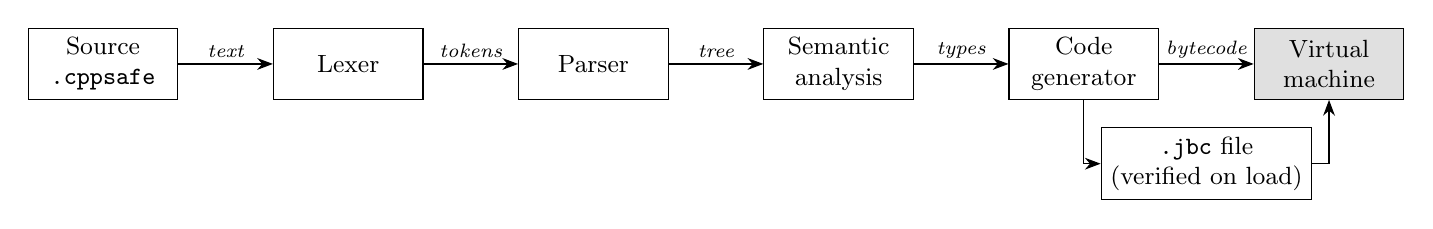
\begin{tikzpicture}[
  stage/.style={draw, rectangle, minimum width=1.9cm, minimum height=0.9cm, align=center, font=\small},
  art/.style={font=\scriptsize\itshape, inner sep=1pt},
  >={Stealth[length=2mm]}]
  \node[stage] (src) {Source\\ \texttt{.cppsafe}};
  \node[stage, right=1.2cm of src] (lex) {Lexer};
  \node[stage, right=1.2cm of lex] (par) {Parser};
  \node[stage, right=1.2cm of par] (sem) {Semantic\\ analysis};
  \node[stage, right=1.2cm of sem] (gen) {Code\\ generator};
  \node[stage, right=1.2cm of gen, fill=black!12] (vm) {Virtual\\ machine};
  \foreach \a/\b/\l in {src/lex/text, lex/par/tokens, par/sem/tree, sem/gen/types, gen/vm/bytecode} {
    \draw[->] (\a) -- node[art, above=1pt] {\l} (\b);
  }
  \node[stage, below=0.8cm of $(gen)!0.5!(vm)$, minimum width=2.6cm] (jbc) {\texttt{.jbc} file\\ (verified on load)};
  \draw[->] (gen.south) |- (jbc.west);
  \draw[->] (jbc.east) -| (vm.south);
\end{tikzpicture}
\caption{Pipeline of the \jscpp\ compiler. Bytecode can be run directly or saved to a \texttt{.jbc} file, which the
loader verifies before the virtual machine runs it.}
\label{fig:pipeline}
\end{figure*}

Figure~\ref{fig:pipeline} shows the pipeline. Table~\ref{tab:loc} gives the size of each part; the whole system is
\res{loc_total} lines of C++17 and uses only the standard library.

\begin{table}[t]
\caption{Source size by component (lines of code).}
\label{tab:loc}
\centering
\begin{tabular}{lr}
\toprule
Component & Lines \\
\midrule
Lexer & 369 \\
Parser and AST & 982 \\
Semantic analysis & 657 \\
Bytecode and code generator & 851 \\
Virtual machine and heap & 563 \\
Common and command line & 216 \\
\midrule
Total & 3{,}638 \\
\bottomrule
\end{tabular}

\end{table}

\subsection{Front end}
The lexer is a hand-written scanner that records a line and column for every token, which later lets errors quote
the source line with a caret. It also rejects values that do not fit in a 32-bit \texttt{int}. The parser is a
recursive-descent parser with one function per precedence level. It rewrites \texttt{for} loops into
\texttt{while} loops, and \texttt{++}, \texttt{--} and compound assignment into plain assignments, but only when
the target has no side effects (a variable, \texttt{a[i]} or \texttt{*p}), so that nothing is evaluated twice.

\subsection{Semantic analysis}
Semantic analysis visits the syntax tree twice. The first pass records the signature of every function, which is
what allows calls before definitions and recursion. The second pass checks each body: types must match exactly,
the left side of an assignment must be a storage location, whole arrays cannot be assigned, and every path of a
non-void function must return. The pass stores the type of every expression and declaration for the code
generator.

\subsection{Code generation}
The code generator assigns each variable of a function its own frame slot, with parameters in the first slots.
It compiles \texttt{\&\&} and \texttt{||} to conditional jumps so the right operand runs only when needed, and it
records the source line of every instruction. Safety instructions are inserted as described in
Section~\ref{sec:safety}.

\subsection{Virtual machine and bytecode}
The machine has an operand stack, a call stack of frames, one array of locals shared by all frames, and a heap
that maps integer handles to objects holding a reference count, a size and the cells. Handles are never reused, so
a stale handle can never name a newer object. The instruction set has \res{loc_opcodes} instructions. A call
instruction names its target by index in a function table. The \texttt{.jbc} file stores every integer as four
little-endian bytes, so the same file runs unchanged on every platform, and a verifier checks every opcode,
constant index, function index, jump target and allocation size when a file is loaded.

%--------------------------------------------------------------------
\section{Safety Mechanisms}
\label{sec:safety}

\subsection{Pointers cannot be forged}
A pointer value can only come from \texttt{new}, from \texttt{nullptr}, or by copying another pointer. Because the
language has no address-of operator, pointer arithmetic or casts, every non-null pointer names a live (or
once-live) heap object. This is the property that makes the run-time checks below sufficient.

\subsection{Null and bounds checks}
Every dereference \texttt{*p} compiles to \texttt{CHECK\_NULL} followed by the load or store, and every
\texttt{a[i]} compiles to \texttt{CHECK\_BOUNDS} followed by the access. For the statement \texttt{*p = a[1];}
the compiler emits:
\begin{lstlisting}
LOAD_LOCAL  0       ; array a
PUSH_CONST  (=1)    ; index
CHECK_BOUNDS        ; 0 <= index < size
LOAD_ARRAY
LOAD_LOCAL  1       ; pointer p
CHECK_NULL          ; pointer is not null
STORE_POINTER
\end{lstlisting}
The access instructions repeat the range test themselves, so hand-written bytecode cannot skip the check. A failed
check stops the machine with a named exception, the source line and the function name, and \jscpp\ exits with
status~1.

\subsection{Automatic reference counting}
\label{sec:arc}
Every heap object carries a reference count. The code generator follows one convention:
\begin{itemize}
\item Each local pointer or array variable owns one reference.
\item \texttt{new} and a call that returns a pointer produce an \emph{owned} value (its count already includes the
      reference being handed over); storing it transfers that reference.
\item Reading a variable produces a \emph{borrowed} value; storing it emits \texttt{INC\_REF}.
\item Pointer arguments are passed as owned references, and the callee releases its parameters when it returns.
\item \texttt{DEC\_REF} is emitted when a variable is reassigned (after the new value is retained, so
      \texttt{p = p} is safe), at the end of every block, and on every \texttt{return}.
\item A pointer result that nobody stores, such as \texttt{make();}, is released immediately.
\end{itemize}
When a count reaches zero the object is freed at once. \texttt{delete p} releases \texttt{p}'s reference and then
sets \texttt{p} to \texttt{nullptr}; other variables that refer to the same object keep it alive, so \texttt{delete}
cannot produce a dangling pointer.

\emph{Why cycles cannot occur.} A cycle needs one heap object to hold a reference to another. Heap cells hold only
\texttt{int} or \texttt{bool} values, because pointers to pointers and arrays of pointers are rejected by the
type rules. References therefore live only in frame slots, and the reference graph between heap objects is empty.
The usual weakness of reference counting does not apply to this subset. This argument rests on the type rules; we
test it but do not prove it formally.

\subsection{Defined arithmetic and bounded resources}
Signed overflow is undefined in C++, so the machine computes \texttt{+}, \texttt{-} and \texttt{*} on unsigned
32-bit values and converts back; the result wraps as in Java. \texttt{INT\_MIN / -1} is handled explicitly and
division by zero raises an exception. The call stack is limited to 1000 frames, the operand stack to 100{,}000
values and the heap to one million live objects, so runaway programs stop with an exception rather than
exhausting the host.

%--------------------------------------------------------------------
\section{Evaluation}
\label{sec:eval}
All numbers in this section were produced by a script (\texttt{collect\_results.py}) that runs the real compiler
and writes JSON files; the text and tables read those files, so no figure was typed by hand. Measurements were made
on a laptop with an \res{cpu} processor running Windows~11, compiled with g++~\res{gpp}; Linux results use
g++~\res{linux_gpp} under WSL. Claims below are \emph{observed} unless stated otherwise.

\subsection{Audit of the first version}
Before extending the system we built its first working version and ran small probe programs against it. We found
\res{audit_total} faults: \res{audit_critical} critical (the feature did not work), \res{audit_high} high
(invalid programs accepted or undefined behaviour) and \res{audit_medium} medium (robustness and usability).
The critical ones were: (i) \texttt{\&\&} and \texttt{||} emitted a jump whose target was never filled in and stayed
at address zero, so \texttt{if (true || false)} never terminated; (ii) parameters were numbered after the locals of
earlier functions, so a call stored its arguments in the wrong slots and a program that should print 42 printed
0; (iii) locals declared at function level were never released, so reference counting freed nothing for them; and
(iv) arrays were never released either. All faults were fixed, and each is covered by a regression test.

\subsection{Test suite}
The suite has \res{tests_total} tests. Each of the \res{tests_examples} example programs is run twice, once from
source and once after saving to and loading from a \texttt{.jbc} file (\res{tests_run} + \res{tests_bytecode}
tests), and the output, exit status and, for the failing demonstrations, the exception text must match exactly.
A further \res{tests_rejected} invalid programs must each be rejected with a specific message
(\res{tests_reject} tests). All \res{tests_total} tests pass on Windows, and all \res{linux_total} pass on Linux.
We also confirmed that the harness reports a failure when an expected output is deliberately changed.

\subsection{Safety outcomes}
Table~\ref{tab:safety} lists \res{safety_demos} small programs, each performing one unsafe action. \res{safety_runtime} are
stopped at run time with an exception, one completes with a defined result, and \res{safety_compile} are rejected
before running.

\begin{table*}[t]
\caption{Result of each unsafe action (observed). ``Line'' is the source line reported.}
\label{tab:safety}
\centering
\small
\begin{tabular}{p{5.6cm}lp{5.6cm}r}
\toprule
Unsafe action & Stage & Result & Line \\
\midrule
Store one past the end of an array & run & \texttt{ArrayIndexOutOfBoundsException} & 7 \\
Read an array at index $-1$ & run & \texttt{ArrayIndexOutOfBoundsException} & 5 \\
Dereference \texttt{nullptr} & run & \texttt{NullPointerException} & 4 \\
Use a pointer after \texttt{delete} & run & \texttt{NullPointerException} & 5 \\
Divide by zero & run & \texttt{DivisionByZeroException} & 2 \\
Recurse without a base case & run & \texttt{StackOverflowException} & 2 \\
Add one to the largest \texttt{int} & run & completes, prints $-2147483648$ & -- \\
Take an address with \texttt{\&} & compile & rejected: compile error & 3 \\
Non-void function that can end without \texttt{return} & compile & rejected: compile error & 1 \\
\bottomrule
\end{tabular}

\end{table*}

\subsection{Memory behaviour}
Of the \res{heap_programs} example programs, \res{heap_clean_programs} finish normally. Together they allocate
\res{heap_clean_allocations} heap objects and free \res{heap_clean_frees}, leaving \res{heap_clean_leaks} alive at
exit. Programs that stop on an exception can leave objects alive at that moment; the machine reclaims them when it
exits. A larger program, \texttt{showcase.cppsafe} (\res{show_source_lines} lines, \res{show_functions} functions,
using recursion, sorting, binary search, pointers, \texttt{delete} and overflow), produces \res{show_tokens} tokens,
a tree of \res{show_ast_nodes} nodes and \res{show_instructions} instructions. Of these, \res{show_check_null}
are \texttt{CHECK\_NULL}, \res{show_check_bounds} are \texttt{CHECK\_BOUNDS}, \res{show_inc_ref} are
\texttt{INC\_REF} and \res{show_dec_ref} are \texttt{DEC\_REF}, all inserted by the compiler. The machine executes
\res{show_executed} instructions, allocates \res{show_allocations} objects and frees \res{show_frees}. The program's
\res{show_printed_values} printed values were also compared with an independent Python implementation of the same
computation (\texttt{verify\_showcase.py}), and all matched.

\subsection{Performance}
\begin{table}[t]
\caption{Wall-clock time in milliseconds (median of \res{bench_reps} runs, including process start-up). Ratio is VM
(Release) divided by native.}
\label{tab:perf}
\centering
\small\setlength{\tabcolsep}{3pt}
\begin{tabular}{lrrrr}
\toprule
Benchmark & Native & VM (Rel.) & VM (def.) & Ratio \\
\midrule
\texttt{fib(27)} & 5 & 29 & 198 & 6$\times$ \\
loop, $3\times10^{6}$ iter. & 6 & 197 & 1526 & 32$\times$ \\
bubble sort, 1500 items & 10 & 165 & 1421 & 17$\times$ \\
\bottomrule
\end{tabular}

\end{table}

We compared the virtual machine with the same algorithm written in C++ and compiled with \texttt{g++ -O2}.
``VM (Rel.)'' is the \jscpp\ binary built in Release mode (\texttt{-O3}); ``VM (def.)'' is the default build without
optimisation flags. All three benchmarks print identical results in the virtual machine and in native code.
Table~\ref{tab:perf} shows that the Release interpreter is \res{ratio_min} to \res{ratio_max} times slower than
native code. Process start-up (\res{startup_vm_ms}~ms for the virtual machine, \res{startup_native_ms}~ms
for the native program) is included in every time, so the true ratio for the shortest benchmark is higher than
shown. Building \jscpp\ itself with optimisation makes it \res{opt_min} to \res{opt_max} times faster than the
default build. We did not compare with the Java Virtual Machine; it was not available on the test machine.

%--------------------------------------------------------------------
\section{Limitations and Threats to Validity}
\begin{itemize}
\item \emph{Evidence, not proof.} The guarantees follow from the type rules and the checks, but we have not proved
      them formally. Our evidence is a hand-written suite, not a fuzzing or differential-testing campaign.
\item \emph{Small language.} There are no structs, strings, global variables or heap arrays, and \texttt{print}
      accepts only an \texttt{int}. The guarantees apply to this subset only.
\item \emph{Exceptions end the program.} The language has no \texttt{try}/\texttt{catch}; a failed check stops the
      program, as an uncaught exception does in Java.
\item \emph{Cost of safety.} The checks are never removed, and the interpreter has no just-in-time compiler.
      The benchmarks are small, run on one machine, and cannot separate the cost of the checks from the cost of
      interpretation.
\item \emph{Audit scope.} The \res{audit_total} faults were found by us on our own first version; other faults may
      remain.
\end{itemize}
Natural next steps are differential fuzzing against native C++, structs with reference-counted fields and a cycle
collector, run-time-sized heap arrays, and removing checks that the compiler can prove unnecessary.

%--------------------------------------------------------------------
\section{Conclusion}
\jscpp\ shows that a compiler and virtual machine small enough to read in an afternoon can turn the most common
C++ memory errors into compile-time rejections or named run-time exceptions, and can reclaim memory exactly with
reference counting. The price is a restricted language and execution that is many times slower than native code.
The audit of the first version also showed how easily such a system can appear to work while its main features
fail, which is why the final system is backed by an automated test suite. The source code, tests and demonstration
programs are available at \url{https://github.com/Vaibhav8075/java-safe-cpp}.

\bibliographystyle{IEEEtran}
\bibliography{references}

\end{document}
